\section{Experiments}
\label{sec:experiments}

We evaluate ZhuLong-SE on EDA-Eval-PyAether, the 158-task real-world PyAether scripting benchmark introduced by ZhuLong~\cite{liu2026zhulong}\footnote{We obtained the benchmark by contacting its authors.}. Each task is a natural-language docstring plus a function signature, and a submission passes only if real sandbox execution satisfies a hidden test (the black-box verifier). The primary model is DeepSeek-V4-Pro-Preview. The human-crafted experience consists of four skills and one rule authored by a senior EDA engineer with extensive experience in PyAether development.
% 我们在EDA-Eval-PyAether上评估ZhuLong-SE；该基准由ZhuLong~\cite{liu2026zhulong}提出，包含158个真实PyAether脚本任务。每个任务由自然语言docstring和函数签名组成，提交仅在真实沙箱执行满足隐藏测试（黑盒验证器）时通过。主要模型为DeepSeek-V4-Pro-Preview。人工编写经验由四条技能和一条规则组成，作者是一位具有丰富PyAether开发经验的高级EDA工程师。

The experiments have two parts. First, on all 158 tasks, we ask whether the enhanced ZhuLong-SE harness outperforms the original ZhuLong across matched LLM backbones and which measured harness components contribute to the gain. Second, after removing human-crafted experience, we ask whether governed self-evolution can match or surpass the human-crafted-experience baseline.
% 实验分为两部分。第一部分在全部158个任务上考察增强后的ZhuLong-SE任务级框架是否在匹配的LLM基座上优于原始ZhuLong，以及哪些可测量的框架组件对增益作出贡献。第二部分移除人工编写经验，考察受治理的自进化能否匹配或超过人工经验基线。

\subsection{Harness Evaluation}
\label{sec:exp_retrieval}

We first evaluate the enhanced task-level harness, with self-evolution disabled throughout this subsection. The complete ZhuLong-SE configuration enables all harness enhancements described in Section~\ref{sec:method}, including full retrieval, documentation enrichment, sandbox isolation, the static checker, and human-crafted experience. We first compare this configuration with the published ZhuLong baseline and then decompose the measured components under the primary backbone. No self-evolved knowledge is injected into any result reported in this subsection. For each comparison, the backbone version and settings other than the harness components under study are aligned with ZhuLong~\cite{liu2026zhulong}. Table~\ref{tab:cross_method} uses the reported ZhuLong results where available.
% 我们首先评估增强后的任务级执行框架，本小节始终禁用自进化。完整的ZhuLong-SE配置启用了第~\ref{sec:method}节所述的全部框架增强，包括完整检索、文档增强、沙箱隔离、静态检查器和人工编写经验。我们首先将该配置与已发表的ZhuLong基线进行比较，随后在主要基座模型上分解可独立测量的组件。本小节报告的所有结果均未注入自进化知识。对于每个基座匹配的比较，除被研究的框架组件外，其余设置均与ZhuLong~\cite{liu2026zhulong}所报告的设置对齐；表~\ref{tab:cross_method}中的ZhuLong结果直接取自该论文，而非由本文重新运行。

Table~\ref{tab:cross_method} compares ZhuLong-SE with ZhuLong on the same backbone versions. Across all the five comparisons, ZhuLong-SE improves by 11.4~pp on DeepSeek-V4-Pro-Preview, 16.4~pp on GLM-5.2, 5.7~pp on Kimi-K2.6, 6.9~pp on DeepSeek-V4-Flash-Preview, and 15.8~pp on Doubao-Seed-2.0-pro. Because self-evolution is disabled, these gains reflect the combined task-level enhancements in Section~\ref{sec:method}. The comparisons indicate transfer across the tested model families, although absolute performance still depends on backbone capability.
% 表~\ref{tab:cross_method}在相同基座版本上比较ZhuLong-SE与ZhuLong。在五组对齐比较中，ZhuLong-SE在DeepSeek-V4-Pro-Preview上提升了11.4个百分点，GLM-5.2上提升16.4个百分点，Kimi-K2.6上提升5.7个百分点，DeepSeek-V4-Flash-Preview上提升6.9个百分点，Doubao-Seed-2.0-pro上提升15.8个百分点。由于自进化被禁用，这些提升反映了第~\ref{sec:method}节所述的全部任务级增强。这些比较表明跨模型族的迁移性，尽管绝对性能仍取决于基座能力。

\begin{table}[ht]
\caption{Harness-only Pass@1 comparison with ZhuLong on aligned backbone versions (158 tasks, one ZhuLong-SE run per model, no self-evolution). }
\label{tab:cross_method}
\setlength{\tabcolsep}{2pt}
\centering
\small
\begin{tabular}{lccr}
\toprule
Model & ZhuLong & ZhuLong-SE & $\Delta$ \\
\midrule
DeepSeek-V4-Pro-Preview   & 81.0\% & 92.4\% & +11.4~pp \\
GLM-5.2                   & 74.7\% & 91.1\% & +16.4~pp \\
Kimi-K2.6                 & 83.5\% & 89.2\% & +5.7~pp \\
DeepSeek-V4-Flash-Preview & 78.5\% & 85.4\% & +6.9~pp \\
Doubao-Seed-2.0-pro       & 55.7\% & 71.5\% & +15.8~pp \\
\bottomrule
\end{tabular}
\end{table}

Each harness configuration is evaluated once because a full 158-task run is costly, and the broad task coverage reduces sensitivity to any single task outcome. Repeated runs are reserved for the smaller validation and challenge-test evaluations.
% 每个框架配置仅评估一次，因为完整的158个任务运行成本高昂。广泛的任务覆盖降低了对单个任务结果的敏感度；因此重复运行仅保留给规模较小的验证集和挑战测试评估。

% \begin{table}[ht]
% \caption{Cross-model generalization: same Full-retrieval, Human-crafted configuration across five LLMs (single run, 158 tasks). Tokens are summed over all tasks.}
% \label{tab:cross_model}
% \centering
% \small
% \begin{tabular}{lcrr}
% \toprule
% Model & Pass@1 & Time & Token \\
% \midrule
% DeepSeek-V4-Pro-Preview   & 92.4\% & 22.5\,h & 114.8\,M \\
% GLM-5.2                   & 91.1\% & 28.0\,h & 128.0\,M \\
% Kimi-K2.6                 & 89.2\% & 22.7\,h & 126.2\,M \\
% DeepSeek-V4-Flash-Preview & 85.4\% & 11.1\,h & 134.0\,M \\
% Doubao-Seed-2.0-pro       & 71.5\% & 7.5\,h  & 28.3\,M \\
% \bottomrule
% \end{tabular}
% \end{table}

We next perform an ablation study on ZhuLong-SE. Because ZhuLong-SE is inherited from ZhuLong, we use progressive rather than leave-one-out ablation to attribute that advantage to the newly added components. Checker \emph{ON} enables the static checker, whereas \emph{OFF} bypasses it. \emph{Semantic-Only} retains \texttt{search\_apis} but disables the keyword tool and BM25 supplement, whereas \emph{Full} enables both tools. \emph{Bare} uses no human-crafted knowledge, whereas \emph{Human} adds four skills and one rule derived from human PyAether development experience rather than the benchmark tasks. DeepSeek-V4-Pro-Preview serves as the fixed inference backbone. Table~\ref{tab:ablation} shows that successive additions raise Pass@1 from 81.0\% to 87.3\% with the checker (+6.3~pp), to 88.6\% with Full retrieval (+1.3~pp), and to 92.4\% with Human experience (+3.8~pp). Each component therefore contributes, with the checker providing the largest stepwise gain. Documentation enrichment and sandbox isolation remain fixed and are evaluated only in the overall harness comparison.
% 由于ZhuLong-SE继承自ZhuLong，我们采用递进式而非逐项移除消融，以归因这一优势来自哪些新增组件。检索层包含两个级别：\emph{Full}（第~\ref{sec:method_retrieval}节）和\emph{Semantic-Only}，后者保留语义\texttt{search\_apis}路径，但禁用专用关键词工具和BM25补充。经验层也包含两个级别：\emph{Bare}不使用人工编写的技能或规则，\emph{Human}则包含四条人工技能和一条规则。这些资产来自PyAether平台开发期间积累的领域知识，并非通过检查或拟合158个基准任务得到，因此不构成测试集泄露。以关闭检查器的Bare、Semantic-Only配置为起点，后续各行依次加入检查器、Full检索和Human经验。
% 依次加入检查器、Full检索和Human经验后，Pass@1从81.0\%提高到87.3\%（+6.3个百分点）、88.6\%（+1.3个百分点）和92.4\%（+3.8个百分点）。各组件均有贡献，其中检查器的单步增益最大。文档增强与沙箱隔离保持固定，仅在整体框架比较中评估。

\begin{table}[ht]
\caption{Progressive harness ablation on the 158-task benchmark (single run, DeepSeek-V4-Pro-Preview).}
\label{tab:ablation}
\centering
\small
\begin{tabular}{lccr}
\toprule
Experience & Retrieval & Checker & Pass@1 \\
\midrule
Bare  & Semantic-Only & OFF & 81.0\% \\
Bare  & Semantic-Only & ON & 87.3\% \\
Bare  & Full          & ON & 88.6\% \\
% Human & Semantic-Only & ON & 89.9\% \\
Human & Full          & ON & 92.4\% \\
\bottomrule
\end{tabular}
\end{table}

% \begin{table}[ht]
% \caption{Retrieval--experience decomposition on the 158-task benchmark (single run, DeepSeek-V4-Pro-Preview). Time is wall-clock per run, and tokens are summed over all tasks.}
% \label{tab:retrieval_ablation}
% \centering
% \small
% \begin{tabular}{lccrr}
% \toprule
% Experience & Retrieval & Pass@1 & Time & Token \\
% \midrule
% Bare  & Semantic-Only & 87.3\% & 15.0\,h & 83.1\,M \\
% Bare  & Full          & 88.6\% & 15.8\,h & 75.3\,M \\
% Human & Semantic-Only & 89.9\% & 17.0\,h & 122.9\,M \\
% Human & Full          & 92.4\% & 22.5\,h & 114.8\,M \\
% \bottomrule
% \end{tabular}
% \end{table}

Task~132 illustrates why the keyword path complements semantic retrieval. The task connects two orthogonal routing paths by placing a via at their intersection and requires constructing several SWIG-wrapped types. With Semantic-Only retrieval, the agent issued natural-language queries but did not retrieve the required type definitions, eventually passing a native tuple where a wrapped object was required. With Full retrieval, the agent queried \texttt{ViaDef}, \texttt{emyPoint}, and \texttt{emyString} through the keyword path, retrieved their construction signatures, and completed the task successfully. This case reflects the intended role of camel-case splitting and exact-fragment matching: they make abbreviation-dense API and type names directly addressable when natural-language similarity is insufficient.
% Task~132说明了关键词路径为何能够补充语义检索。该任务需要在两条正交布线路径的交点放置过孔，并构造多个SWIG封装类型。在Semantic-Only检索下，智能体发出自然语言查询，但未检索到所需的类型定义，最终在需要封装对象的位置传入了原生tuple。在Full检索下，智能体通过关键词路径查询\texttt{ViaDef}、\texttt{emyPoint}和\texttt{emyString}，获得其构造签名并成功完成任务。该案例体现了驼峰拆分和精确片段匹配的预期作用：当自然语言相似度不足时，它们使缩写密集的API与类型名称可以被直接检索。

Finally, we characterize the residual failures of the enhanced harness. Figure~\ref{fig:failure_types} aggregates the 111 failed tasks across the five ZhuLong-SE backbone runs in Table~\ref{tab:cross_method}. \texttt{AssertionError} accounts for 54.1\% of these failures: the generated program reaches the hidden verifier without an uncaught API or type error, but its result violates a tested property. Such semantic or result-level errors lie outside the static checker's declared scope, which targets deterministic API misuse rather than hidden functional correctness. This analysis therefore characterizes the remaining failure frontier rather than directly measuring checker recall. Since the task-level harness still solves each task independently, these residual errors motivate the next subsection's evaluation of whether validated knowledge distilled from prior traces can improve later tasks.
% 最后，我们分析增强框架的剩余失败。图~\ref{fig:failure_types}汇总了表~\ref{tab:cross_method}中ZhuLong-SE在五个基座模型上的111个失败任务。其中，\texttt{AssertionError}占54.1\%：生成程序在没有未捕获API或类型错误的情况下到达隐藏验证器，但其结果违反了被测试的属性。这类语义或结果层面的错误超出了静态检查器的既定范围；检查器针对的是确定性API误用，而非隐藏的功能正确性。因此，该分析刻画的是剩余失败边界，而不是对检查器召回率的直接测量。由于任务级框架仍独立解决每个任务，这些剩余错误进一步引出下一小节：由先前轨迹蒸馏并经过验证的知识能否改善后续任务。

\begin{figure}[ht]
\centering
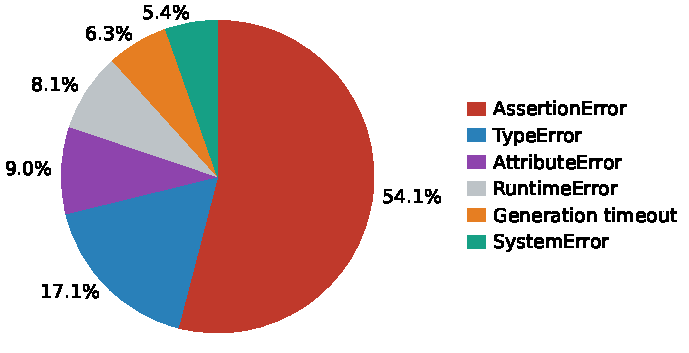
\includegraphics[width=\columnwidth]{figures/failure_type_distribution.pdf}
\caption{Residual failure types of ZhuLong-SE across five LLM backbones on the 158-task benchmark (111 failures aggregated).}
\label{fig:failure_types}
\end{figure}

\subsection{Self-Evolution}
\label{sec:exp_selfev}

To evaluate self-evolution without ceiling effects—the Bare agent already passes 87\% of the 158 tasks—and to support held-out gating, we adopt an instance-disjoint \emph{challenge split} (train~98 / val~20 / test~40), in the spirit of EvoAgentBench's ability-supported yet instance-disjoint split~\cite{gao2026evoagentbench}. The split is stratified so that the test set concentrates more discriminative tasks, identified by testbench code length and the number of unique APIs used. Because the validation and test sets are small, every self-evolution evaluation is the mean of \textbf{five} independent runs with its standard deviation.
% 为在没有天花板效应的情况下评估自进化——Bare智能体已通过158个任务中87\%——并支持留出门控，我们采用实例不相交的\emph{挑战划分}（训练98/验证20/测试40），遵循EvoAgentBench的能力支撑但实例不相交划分的精神~\cite{gao2026evoagentbench}。该划分经过分层，使测试集集中于更具区分度的任务——以测试台代码长度和使用的唯一API数量为标识。由于验证集和测试集较小，每个自进化评估均为\textbf{五次}独立运行的平均值及其标准差。

Table~\ref{tab:sevolution} reports test Pass@1 across rounds, against the Bare baseline (no evolved knowledge) and the Human baseline. Self-evolution clears the Bare baseline by +14.0~pp (66.0\%$\to$80.0\%) and surpasses the Human baseline (80.0\% vs.\ 77.5\%) at Round~2, after which Round~3 regresses to 75.5\%. The validation trend is consistent: validation peaks at Round~2 (88.0\%) and drops at Round~3 (80.0\%), so the gate accepts Rounds~1 and~2 but rejects Round~3, rolling back its 52 new entries and freezing the knowledge base at Round~2 (334 entries, 20 skills). Crucially, the test trend agrees with validation—Round~3 regresses on both (75.5\% vs.\ 80.0\%)—confirming the gate's rejection reflects genuine overfitting, not a validation-specific artifact. Round~2 also has the smallest observed run-to-run spread ($\pm$3.1), below the Human baseline's $\pm$5.3.
% 表~\ref{tab:sevolution}报告了各轮次测试Pass@1，对比Bare基线（无进化知识）和Human基线。自进化以+14.0个百分点（66.0\%$\to$80.0\%）超越Bare基线，并在第2轮超越Human基线（80.0\%对比77.5\%），之后第3轮退步至75.5\%。验证趋势一致：验证集在第2轮达到峰值（88.0\%），在第3轮下降（80.0\%），因此门控接受第1轮和第2轮但拒绝第3轮，回滚其52条新条目并将知识库冻结在第2轮（334条条目，20条技能）。关键的是，测试趋势与验证一致——第3轮在两者上均退步（75.5\%对比80.0\%）——确认门控的拒绝反映的是真正的过拟合而非验证集特有的假象。第2轮还具有观测到的最小跨运行波动（$\pm$3.1），低于Human基线的$\pm$5.3。

\begin{table}[ht]
\caption{Self-evolution on the challenge test set (40 tasks, 5 runs each, DeepSeek-V4-Pro-Preview). ``Patterns'' is the L1 entry count, ``skills'' are auto-distilled. The held-out gate accepted Rounds~1 and~2, and rejected Round~3.}
\label{tab:sevolution}
\setlength{\tabcolsep}{2.5pt}
\centering
\small
\begin{tabular}{lcccc}
\toprule
Knowledge & Patterns & Skills & Pass@1 (test) & Pass@1 (val) \\
\midrule
Bare          & 0   & 0  & 66.0\%$\pm$7.2  & --- \\
Round~1 & 256 & 16 & 78.0\%$\pm$9.9  & 81.0\%$\pm$8.2 \\
Round~2 & 334 & 20 & \textbf{80.0\%}$\pm$3.1  & 88.0\%$\pm$2.7 \\
Round~3 & 386 & 25 & 75.5\%$\pm$6.7  & 80.0\%$\pm$3.5 \\
\midrule
Human Baseline & --- & 4  & 77.5\%$\pm$5.3  & --- \\
\bottomrule
\end{tabular}
\end{table}

To examine the write-side gates under a fixed input, we freeze the 24 distinct failed-task traces accumulated across post-split batches and re-run the offline reflection chain with each gate toggled. This avoids the cost and sparse signal of full end-to-end ablation (13 hours per round), following Trace2Skill's shared-trace-pool design~\cite{ni2026trace2skill}. Test failure traces serve only as offline-reflection inputs, and knowledge produced from them is never injected into test evaluation. Table~\ref{tab:se_write_ablation} reports the resulting L1 entry counts. Because reflection is not fully deterministic, we interpret only gate-shaped changes rather than one-entry differences.
% 为考察每个门控的贡献，我们通过开关每个写入侧门控（第~\ref{sec:se_distill}至~\ref{sec:se_govern}节介绍的真值锚定、失败路由、矛盾路径、范围边界和证伪过滤）来进行消融。对每个门控进行完整端到端消融成本高昂（每轮13小时）且信号稀疏，因为失败触发的门控每轮仅作用于少数任务。遵循Trace2Skill~\cite{ni2026trace2skill}的共享轨迹池设计，我们冻结在后划分批次中积累的24条不同失败任务轨迹，仅重新运行离线反思链，每次切换一个门控，测量知识质量而非端到端Pass@1。测试失败轨迹仅作为此离线反思的输入，由它们产生的任何知识均不注入任何测试评估，因此其包含不构成测试集泄露。表~\ref{tab:se_write_ablation}报告条目数量。由于离线反思LLM并非完全确定性，ON列在各门控间存在±1的差异；我们仅读取门控带来的增量变化，而非单条目的差异。

\begin{table}[ht]
\caption{Write-side gate ablation on the frozen 24-task failure trace pool.
``ON'' and ``OFF'' report L1 entry counts.}
\label{tab:se_write_ablation}
\centering
\begin{tabular}{lcc}
\toprule
Gate & ON & OFF \\
\midrule
Ground-Truth Anchoring   & 37 & 48 \\
Contradiction Path       & 37 & 54 \\
Routing                  & 36 & 37 \\
Scope Boundary           & 36 & 36$^{*}$ \\
Disconfirmation Filter   & 37 & 37$^{\dagger}$ \\
\bottomrule
\end{tabular}

\vspace{2pt}
{\footnotesize\raggedright
$^{*}$ Affects entry content rather than count.
$^{\dagger}$ Inactive because the threshold requires disconfirmation
across at least two batches.\par}
\end{table}

Ground-truth anchoring has the clearest observed effect: without it, 12 of 24 tasks yield at least one falsely verified entry because the trace's self-reported success is trusted. The net count rises by 11 rather than 12 because one such task produces no entry under correct anchoring. Disabling the contradiction path produces 17 additional entries by mining stale, already-repaired errors, while disabling routing sends failed tasks to the success branch and produces no pitfalls. These entry-count results characterize how the three gates alter reflection output. They do not constitute an end-to-end quality comparison.

The remaining two write-side gates cannot be evaluated by this design. Scope-boundary reflection changes the preconditions and constraints recorded within an entry rather than the entry count, so the reported metric cannot identify its effect. The disconfirmation filter removes an entry only after disconfirmation in at least two batches; no entry can reach that threshold in this single-round replay. Their value therefore remains unverified here and requires content-level assessment and multi-round accumulation, respectively.
% 消融实验分离了各门控的作用。真值锚定是最强的：没有它，24个任务中有12个产生至少一条假阳性已验证条目，因为轨迹的自报告成功被信任。净条目数增加了11条而非12条，因为其中一个任务在正确锚定下不会产生任何条目。禁掉矛盾路径通过挖掘陈旧、已修复的错误额外产生了17个条目；禁掉路由则将所有失败任务送入成功分支，不产生陷阱。剩余两项写侧门控无法通过该设计评估。范围边界反思改变的是条目内记录的前提条件和约束，而非条目数量，因此报告的指标无法识别其作用。证伪过滤器仅在条目于至少两个批次中被证伪后才移除；在此单轮重放中没有任何条目能达到该阈值。因此，它们的价值在此尚未得到验证，分别需要内容级评估和多轮累积来检验。

We also ablate each of the four read-side mechanisms from Section~\ref{sec:se_read} (names-only pre-injection, docstring generalization, problem-side embedding, and the decision not to pre-inject pitfalls) by freezing the Round~2 knowledge and varying the injection configuration, then re-running the agent on validation (baseline 88.0\%$\pm$2.7). Table~\ref{tab:se_read_ablation} isolates each. Pre-injecting pitfalls is the most harmful ($-$8.0~pp): a task's description does not predict which API it will misuse, so a recalled pitfall is usually off-target, confirming the choice to route pitfalls through the runtime query instead. Docstring generalization ($-$6.3~pp when disabled) and names-only injection ($-$4.7~pp when full-sequence injection is used) each contribute—the former because disabling it breaks the query-embedding symmetry, the latter because a full call sequence over-specifies and misleads. The embedding strategy (embedding the problem summary vs.\ the solution text) shows no measurable effect here, which we attribute to names-only injection: under this reduction, the retrieved content is the same regardless of embedding, so the embedding choice is dominated by the names-only reduction. The problem-side embedding is therefore justified by its anti-leakage role rather than by a measurable Pass@1 gain in this configuration.
% 我们还通过冻结第2轮知识并改变注入配置，在验证集上重新运行智能体，对第~\ref{sec:se_read}节引入的四项读取侧机制（仅名称预注入、文档字符串泛化、问题侧嵌入、不预注入陷阱的决策）分别进行消融（基线88.0\%$\pm$2.7）。表~\ref{tab:se_read_ablation}分别隔离了各项。预注入陷阱是最有害的（$-$8.0个百分点）：任务描述无法预测它将误用哪个API，因此召回的陷阱通常偏离目标，证实了将陷阱路由到运行时查询而非预注入的决策。文档字符串泛化（禁用时$-$6.3个百分点）和仅名称注入（使用完整序列注入时$-$4.7个百分点）各有贡献——前者因为禁用它打破了查询-嵌入对称性，后者因为完整调用序列过度具体化并产生误导。嵌入策略（嵌入问题摘要而非解决方案文本）在此没有显示可测量效果，我们将其归因于仅名称注入：在这种缩减下，无论条目基于什么嵌入，检索到的内容都是相同的，因此嵌入选择被仅名称缩减所主导。问题侧嵌入因此由其反泄漏作用而非在此配置中可测量的Pass@1增益所证明。

\begin{table}[ht]
\caption{Read-side injection ablation, frozen Round~2 knowledge, validation (20 tasks, 5 runs). Each row varies one mechanism away from the full system (baseline 88.0\%$\pm$2.7).}
\label{tab:se_read_ablation}
\centering
\small
\begin{tabular}{lcc}
\toprule
Configuration & Pass@1 (val) & $\Delta$ \\
\midrule
Full System (Baseline)        & 88.0\%$\pm$2.7 & --- \\
Pitfall Pre-Injection         & 80.0\%$\pm$5.0 & $-8.0$~pp \\
Docstring Generalization Off  & 81.7\%$\pm$5.8 & $-6.3$~pp \\
Full-Sequence Injection       & 83.3\%$\pm$5.8 & $-4.7$~pp \\
Embed Solution (Not Problem)  & 88.0\%$\pm$2.7 & $0$~pp \\
\bottomrule
\end{tabular}
\end{table}
